\documentclass[tikz,border=8pt]{standalone}

\usepackage[T1]{fontenc}
\usepackage{lmodern}
\usetikzlibrary{arrows.meta,calc,positioning}

\definecolor{RdgBlue}{HTML}{174A8B}
\definecolor{RdgBlueFill}{HTML}{EDF4FD}
\definecolor{AuthPurple}{HTML}{68449A}
\definecolor{AuthFill}{HTML}{F4EFFA}
\definecolor{QueryTeal}{HTML}{087E78}
\definecolor{QueryFill}{HTML}{EAF8F6}
\definecolor{CreateOrange}{HTML}{B45A18}
\definecolor{CreateFill}{HTML}{FFF3E9}
\definecolor{CareGreen}{HTML}{397447}
\definecolor{CareFill}{HTML}{EDF7EF}
\definecolor{Ink}{HTML}{20242A}
\definecolor{Muted}{HTML}{5D6570}
\definecolor{Rule}{HTML}{C9D0D8}
\definecolor{Panel}{HTML}{F7F9FB}

\begin{document}
\sffamily
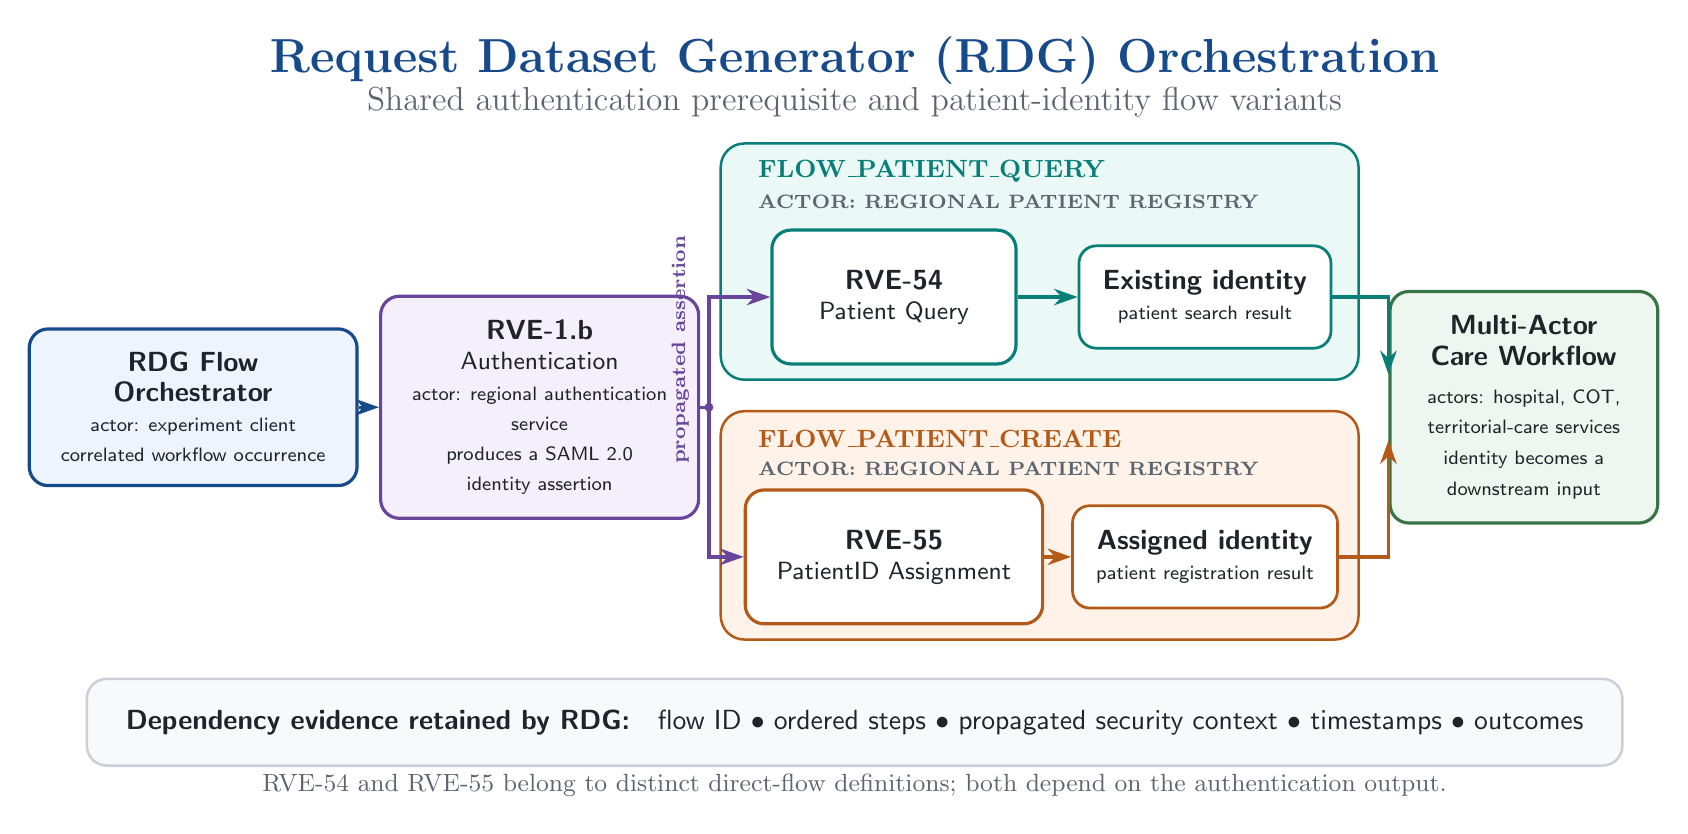
\begin{tikzpicture}[
    font=\sffamily,
    flow/.style={-{Stealth[length=3mm,width=2.1mm]}, line width=1.2pt},
    process/.style={
        rounded corners=2.4mm,
        minimum width=34mm,
        minimum height=17mm,
        align=center,
        line width=1.15pt,
        inner xsep=4mm,
        inner ysep=3mm,
        text=Ink
    },
    output/.style={
        rounded corners=2.2mm,
        minimum width=32mm,
        minimum height=13mm,
        align=center,
        line width=1pt,
        inner xsep=3mm,
        inner ysep=2.5mm,
        text=Ink
    },
    lane/.style={rounded corners=3mm, line width=0.9pt},
    actor/.style={font=\scriptsize\bfseries, text=Muted},
    meta/.style={font=\small, text=Muted, align=center}
]

% Heading
\node[font=\bfseries\LARGE, text=RdgBlue] at (10.25,9.75)
    {Request Dataset Generator (RDG) Orchestration};
\node[font=\large, text=Muted] at (10.25,9.22)
    {Shared authentication prerequisite and patient-identity flow variants};

% RDG orchestration layer
\node[process, draw=RdgBlue, fill=RdgBlueFill] (rdg) at (1.85,5.35)
    {\textbf{RDG Flow}\\[-0.4mm]
     \textbf{Orchestrator}\\[-0.4mm]
     {\scriptsize actor: experiment client}\\[-0.4mm]
     {\scriptsize correlated workflow occurrence}};

% Shared authentication prerequisite
\node[process, draw=AuthPurple, fill=AuthFill] (auth) at (6.25,5.35)
    {\textbf{RVE-1.b}\\[-0.4mm]
     {\small Authentication}\\[-0.2mm]
     {\scriptsize actor: regional authentication}\\[-0.4mm]
     {\scriptsize service}\\[-0.4mm]
     {\scriptsize produces a SAML 2.0}\\[-0.4mm]
     {\scriptsize identity assertion}};

\draw[flow, draw=RdgBlue] (rdg.east) -- (auth.west);

% Flow variant panels
\filldraw[lane, fill=QueryFill, draw=QueryTeal]
    (8.55,5.70) rectangle (16.65,8.70);
\node[anchor=west, font=\small\bfseries, text=QueryTeal] at (8.90,8.35)
    {FLOW\_PATIENT\_QUERY};
\node[anchor=west, actor] at (8.90,7.96) {ACTOR: REGIONAL PATIENT REGISTRY};

\filldraw[lane, fill=CreateFill, draw=CreateOrange]
    (8.55,2.40) rectangle (16.65,5.30);
\node[anchor=west, font=\small\bfseries, text=CreateOrange] at (8.90,4.95)
    {FLOW\_PATIENT\_CREATE};
\node[anchor=west, actor] at (8.90,4.57) {ACTOR: REGIONAL PATIENT REGISTRY};

\node[process, minimum width=31mm, draw=QueryTeal, fill=white] (query) at (10.75,6.75)
    {\textbf{RVE-54}\\[-0.4mm]{\small Patient Query}};
\node[output, draw=QueryTeal, fill=white] (queryout) at (14.70,6.75)
    {\textbf{Existing identity}\\[-0.4mm]{\scriptsize patient search result}};
\draw[flow, draw=QueryTeal] (query.east) -- (queryout.west);

\node[process, minimum width=31mm, draw=CreateOrange, fill=white] (create) at (10.75,3.45)
    {\textbf{RVE-55}\\[-0.4mm]{\small PatientID Assignment}};
\node[output, draw=CreateOrange, fill=white] (createout) at (14.70,3.45)
    {\textbf{Assigned identity}\\[-0.4mm]{\scriptsize patient registration result}};
\draw[flow, draw=CreateOrange] (create.east) -- (createout.west);

% Authentication output is propagated into either selected flow variant.
\coordinate (fork) at (8.40,5.35);
\draw[line width=1.2pt, draw=AuthPurple] (auth.east) -- (fork);
\fill[AuthPurple] (fork) circle (1.6pt);
\draw[flow, draw=AuthPurple] (fork) |- (query.west);
\draw[flow, draw=AuthPurple] (fork) |- (create.west);
\node[font=\scriptsize\bfseries, text=AuthPurple, rotate=90, anchor=south]
    at (8.27,6.08) {propagated assertion};

% Both identity outcomes feed the wider care workflow.
\node[process, minimum width=34mm, minimum height=23mm,
      draw=CareGreen, fill=CareFill] (care) at (18.75,5.35)
     {\textbf{Multi-Actor}\\[-0.2mm]
     \textbf{Care Workflow}\\[0.5mm]
     {\scriptsize actors: hospital, COT,}\\[-0.3mm]
     {\scriptsize territorial-care services}\\[-0.3mm]
     {\scriptsize identity becomes a}\\[-0.3mm]
     {\scriptsize downstream input}};
\draw[flow, draw=QueryTeal] (queryout.east) -| ($(care.west)+(0,0.42)$);
\draw[flow, draw=CreateOrange] (createout.east) -| ($(care.west)+(0,-0.42)$);

% Trace evidence band and implementation-faithfulness note.
\node[draw=Rule, fill=Panel, rounded corners=2.5mm, line width=0.9pt,
      minimum width=195mm, minimum height=11mm, align=center, text=Ink]
      at (10.25,1.35)
    {\textbf{Dependency evidence retained by RDG:}\quad
     flow ID $\bullet$ ordered steps $\bullet$ propagated security context $\bullet$
     timestamps $\bullet$ outcomes};
\node[meta] at (10.25,0.55)
    {RVE-54 and RVE-55 belong to distinct direct-flow definitions; both depend on the authentication output.};

\end{tikzpicture}
\end{document}
